\section{L'implémentation de la physique / Modélisation d'un système de dynamique de véhicule}\label{sec:l'implementation-de-la-physique-/-modelisation-d'un-systeme-de-dynamique-de-vehicule}
\subsection{Introduction}\label{subsec:introduction}
Pour représenter la relation entre un véhicule et la route d'une manière se rapprochant de la réalité, nous avons donc dû implémenter des phénomènes physiques venant des sciences de l'ingénieur. De plus, comme l'étude et la représentation d'un système  de dynamique de véhicule est une tâche plutôt difficile, nous avons décidé de procéder de manière itérative. Tout d'abord, le but était d'avoir une implémentation très basique d'un système de dynamique,  puis une fois celui-ci fonctionnel, d'itérer ce système pour intégrer des phénomènes plus délicats à implémenter, puis d'encore itérer sur ce système, etc.
Ceci nous a mené à un plan en 5 étapes.
Premièrement, implémenter les lois de Newton pour la dynamique du véhicule, puis implémenter un modèle bicycle simplifié, pour ensuite pouvoir représenter les forces sur les pneus et modéliser les glissements, et finalement pouvoir simuler les limites du pneumatique.
Nous allons maintenant vous détailler les principes physiques et l'implémentation que nous avons fournis pour chacune de ces étapes :

\subsection{Implémentation des lois de Newton pour la dynamique du véhicule}\label{subsec:implementation-des-lois-de-newton-pour-la-dynamique-du-vehicule}

Comme base de notre projet, nous avons donc commencé par implémenter la première Loi de Newton qui est le principe d'inertie, elle stipule que tout corps conservera son état de repos ou de mouvement rectiligne uniforme dans lequel il se trouve, à moins qu'une force ne soit appliquée sur ce corps. Ainsi, un système ou corps quelconque ne peut pas se déplacer à moins qu'une force ne lui soit appliquée. Et c'est pareil pour qu'un système passe d'un état de mouvement à un état arrêté.
Dans notre implémentation, cette loi est traduite par le fait que si aucune force n'agit sur le véhicule, alors ses vitesses vont rester nulles (ou constantes si le véhicule est initialisé avec une vitesse).
Pourquoi et comment avons-nous implémenté cette loi ?
Rappelons d'abord que l'équation fondamentale de la dynamique est donnée par :
$$F = m \ .\  a$$
Avec :
\begin{itemize}
    \item $F$ la force appliquée sur le corps,
    \item $m$ la masse du corps,
    \item $a$ l'accélération résultante.
\end{itemize}

Dans notre code, nous avons appliqué cette relation en calculant les accélérations $a_x$ et $a_y$ du véhicule à partir des forces appliquées :


\begin{lstlisting}[style=CStyle,label={lst:void_computeTranslation}]
void computeTranslation(const double Fx, const double Fy, double& ax, double& ay) {
    ax = Fx / m;
    ay = Fy / m;
}
\end{lstlisting}

Ici si $F_x = 0$ et $F_y = 0$, alors $a_x$ et $a_y$, s'annulent, ce qui signifie que les vitesses restent constantes conformément au principe d'inertie.
Cependant, dès qu'on applique une force sur un objet, on génère une accélération. Cette accélération va alors modifier la vitesse de l'objet, et, comme la position est liée à la vitesse de l'objet, alors, elle évoluera dans le temps. Ce processus est décrit par des équations différentielles. Dans notre cas, nous aurons :
$$\frac{d v_x}{dt} = a_x, \quad \frac{d v_y}{dt} = a_y, \quad \frac{d r}{dt} = r_{\dot{}}$$
où $v_x$ et $v_y$ représentent les composantes de la vitesse et $r$ le lacet, l'orientation, du véhicule.

Cependant, comme notre simulateur est en temps réel, résoudre ces équations à chaque itération demanderait de nombreux cycles CPU, alors pour préserver leur usage, nous utilisons une méthode numérique, celle qui est la plus simple et efficace : la \textbf{méthode d'Euler explicite}.

Cette méthode repose sur le fait que la dérivée d'une variable $x$ notée $\dot{x}$ reste constante sur un petit intervalle de temps $dt$. Donc, on peut approximer son évolution par :
$$x(t+dt) \approx x(t) + \dot{x}(t) \times dt$$
Dans la première implémentation de notre simulateur, nous utilisons donc cette formule pour mettre à jour les vitesses et l'orientation de la voiture :
\\



\begin{itemize}
    \item \textbf{Pour la vitesse sur l'axe $x$ :}
    $$v_x(t+dt) = v_x(t)+a_x(t)\times(dt)$$
    \item \textbf{Pour la vitesse sur l'axe $y$ :}
    $$v_y(t+dt) = v_y(t)+a_y(t)\times(dt)$$
    \item \textbf{Pour l'orientation $r$ :}
    $$r(t+dt) = r(t)+\dot{r}(t)\times(dt)$$
\end{itemize}

\begin{center}
    Formules disponibles sur ~\cite{euler_explicite}:
\end{center}

Ici, on utilise $a_x(t)$, car c'est la dérivée de $v_x(t)$ par rapport au temps.
C'est la même chose pour $a_y(t)$ qui résulte de $a_y(t)$.
Ensuite, pour trouver $\dot{r}(t)$, qui est l'accélération angulaire, on applique la loi de la dynamique de rotation angulaire qui est la suivante :
$$I\dot{r}(t) = \texttt{torque}$$
où $I$ est le moment d'inertie de l'objet.
En isolant $\dot{r}(t)$, on obtient :
$$\dot{r}(t)= \frac{\texttt{torque}}{I}$$
Nous calculons cette valeur via un appel à la fonction \texttt{computeYawAcceleration(torque);} où cette relation est implémentée.

Grâce à cela, l'état de notre véhicule est mis à jour en obtenant une approximation de la solution des équations différentielles, plutôt que de les résoudre, ce qui prendrait plus de temps de calcul.
Cependant, la précision de la méthode d'Euler dépend forcément de la taille du pas qu'on lui donne ($dt$), et c'est la même chose pour des systèmes plus complexes. Dans ces cas-ci, cette méthode produira alors des erreurs significatives et la simulation deviendra instable. C'est pourquoi, plus tard dans l'implémentation de notre physique, nous avons choisi d'implémenter une méthode plus fiable dans ces cas-ci.

Ensuite, pour valider le bon fonctionnement des principes physiques que nous avons décrit et implémenté, nous avons réalisé une simulation de 10 secondes (avec un pas de 0,1 s), et avons utilisé \textbf{\gls{gnuplot}} pour visualiser les résultats obtenus et observer si le résultat obtenu est celui attendu. Voici la manière dont nous initialisons notre objet voiture, et indiquons la démarche à suivre pour avoir une simulation sur 10 secondes :

\begin{lstlisting}[style=CStyle,label={lst:void_simulation_etape1}]
void simulation_etape1() {
    // Initialisation du vehicule (mass=1700 kg, dist_cog_front_axle=1.5 m, dist_cog_rear_axle=1.5 m)
    OldVehicle myVehicle(1700.0, 1.5, 1.5);

    // Parametres de simulation
    double Fx = 500.0;       // Force longitudinale (N)
    double Fy = 200.0;       // Force laterale (N)
    double torque = -150.0;  // Moment de lacet (Nm)
    double dt = 0.1;         // Pas de temps (s)
    int steps = 10000;       // Simulation sur 10 secondes

    // Vecteurs pour stocker les donnees : paire (temps, valeur)
    std::vector<std::pair<double, double>>vx_data, vy_data, r_data;

    // Simulation : enregistrement des etats a chaque pas de temps
    for (int i = 0; i <= steps; ++i) {
        vx_data.push_back({t, myVehicle.vx});
        vy_data.push_back({t, myVehicle.vy});
        r_data.push_back({t, myVehicle.lacet});
        myVehicle.update(dt, Fx, Fy, torque);
    }
    // ... Plot des donnees stockees dans les vecteurs avec Gnuplot

}
\end{lstlisting}

{\LARGE Question => Doit-on ajouter la partie code \gls{gnuplot} à la figure précédente ?}

Les graphiques donnés par notre implémentation donnent alors :

\begin{center}
    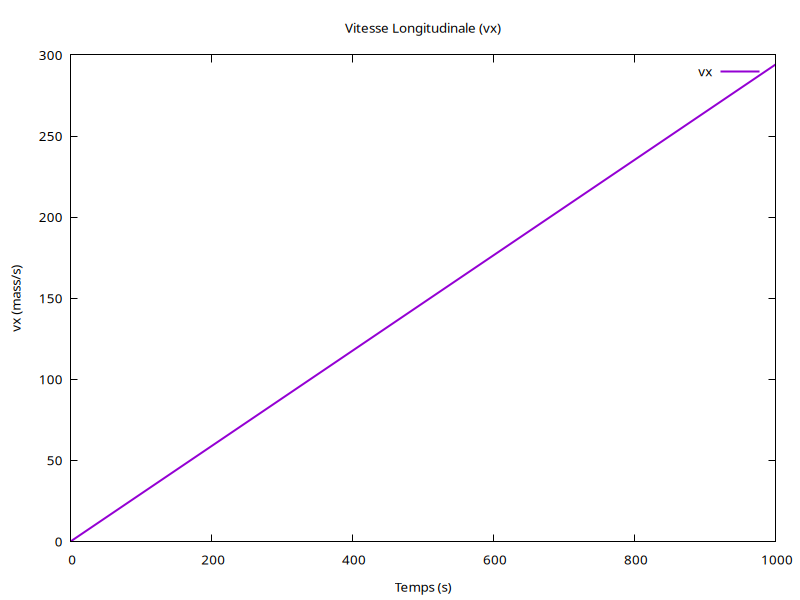
\includegraphics[width=0.70\linewidth]{resources/Plots/Etape1/vx}
    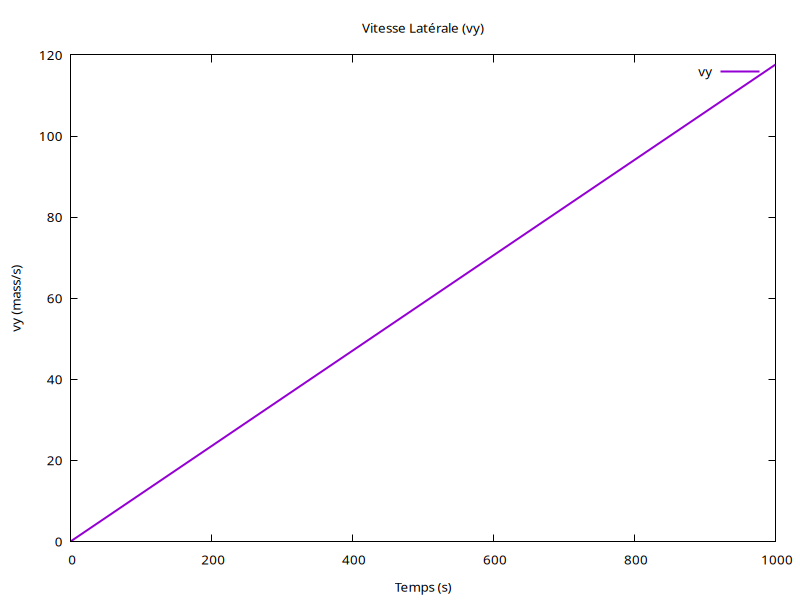
\includegraphics[width=0.70\linewidth]{resources/Plots/Etape1/vy}
    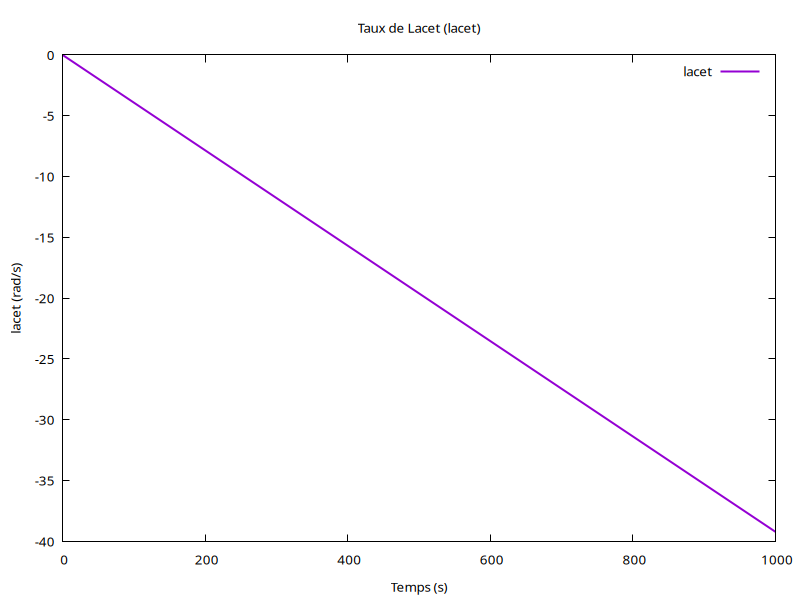
\includegraphics[width=0.70\linewidth]{resources/Plots/Etape1/lacet}
\end{center}

\begin{itemize}
    \item \textbf{Graphique de la vitesse longitudinale ($vx$)} : Sur ce premier graphique, on observe bien que l'évolution de la vitesse sur l'axe $y$, se traduit par l'application de la force longitudinale ($ F = m \cdot a $). Et nous avons donc une accélération constante, ce qui mène à une augmentation linéaire de $vx$ au fil du temps.

    \item \textbf{Graphique de la vitesse latérale ($vy$)} : De même, le graphique représentant $vy$ permet d'observer l'effet de la force latérale appliquée.

    \item \textbf{Graphique du taux de lacet ({$\texttt{lacet}$})} : Et dernièrement, ce graphique-ci nous permet de voir l'évolution de l'orientation du véhicule. Grâce à la loi de la dynamique de rotation ($I\dot{r} = \texttt{torque}$), nous constatons que l'accélération angulaire est directement proportionnelle au couple appliqué, ce qui se traduit par une variation linéaire de $\texttt{lacet}$ au fil du temps.
\end{itemize}

\subsection{Le modèle Bicycle simplifié}
\subsubsection{Explication du modèle Bicycle}
Après avoir implémenté ces phénomènes physiques de base, nous devions rajouter une façon de pouvoir contrôler notre véhicule de manière réaliste. C'est pourquoi nous avons choisi d'implémenter le \textbf{modèle Bicycle simplifié}. C'est un modèle couramment utilisé en dynamique des véhicules, plutôt que de traiter séparément les quatre roues d'un véhicule, il regroupe les roues avant en une seule roue, et fait de même pour les roues arrière. En procédant de cette façon, nous pouvons capturer les comportements dynamiques des pneus d'un véhicule tout en réduisant la complexité des équations utilisées. Comme le but de cette partie était de pouvoir calculer la trajectoire d'un véhicule, nous avons utilisé le modèle bicycle pour trouver l'angle de glissement des pneus, ainsi que pour trouver les forces appliquées sur ceux-ci, pour pouvoir modéliser la trajectoire.

Mais qu'est-ce que l'\textbf{angle de glissement} ? L'angle de glissement est l'angle formé entre la direction réelle d'un pneu et l'orientation de la roue. Il est induit par les forces latérales lors d'un virage. Plus cet angle est grand, plus les forces latérales appliquées sur le pneu sont grandes. Chaque pneu a, en fonction de son état et de la condition de la route (et son revêtement) sur laquelle il se trouve, une limite d'adhérence au-delà de laquelle il ne peut plus maintenir un contact optimal avec la route. Alors, le pneu perd son efficacité et commence à déraper. Cet angle a une grande importance dans la dynamique des véhicules, car il influence leur stabilité et
leur comportement en virage.
C'est en implémentant cette limite, plus tard dans notre modèle, que nous avons pu simuler le comportement de sous-virage et de survirage.
Dans l'illustration ci-dessous, l'angle de glissement est $\alpha$.
\begin{figure}[h]
    \centering
    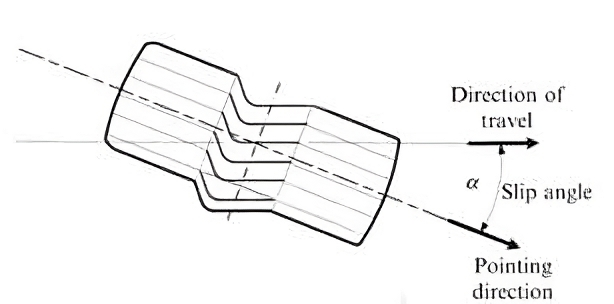
\includegraphics[width=0.5\textwidth]{resources/Plots/Etape2/slip-angle}
    \caption{Illustration de l'angle de glissement. Image tirée de \cite{slip-angle}.}
    \label{fig:bicycle_model}
\end{figure}

\subsubsection{Implémentation du modèle Bicycle}
Premièrement, nous devons calculer les angles de glissement, ce qui se fait avec les formules suivantes :

\begin{itemize}
    \item Pour l'essieu avant (\texttt{alpha\_F} dans notre code) :
    $$\alpha_F = \delta - \frac{(a \dot{\theta}+V_{\xi})}{V_\eta}$$
    \item Pour l'essieu arrière (\texttt{alpha\_R} dans notre code) :
    $$\alpha_R = \frac{(b \dot{\theta}+V_{\xi})}{V_\eta} $$

    Avec :\\
    $\delta$ = L'angle de braquage, \\
    $a$ = Distance entre le \textbf{centre de gravité} et l'\textbf{essieu avant},\\
    $b$ = Distance entre le \textbf{centre de gravité} et l'\textbf{essieu arrière},\\
    $\theta$ = La vitesse de \textbf{lacet}, \\
    $V_\xi$ = La vitesse \textbf{latérale}, \\
    $V_\eta$ = La vitesse \textbf{longitudinale}. \\
    \center{\text{(Formules tirées de \cite{vtech})}}
\end{itemize}

Dans la première étape, nous avions déjà tous ces paramètres, sauf $\delta$, nous avons donc rajouté une variable \texttt{delta}, dans notre objet qui représente donc l'angle de braquage de la voiture.
%Ces deux formules mathématiques se traduisent donc dans notre code par :
%
%\begin{lstlisting}[style=CStyle,label={lst:code_updatebicycle}]
%void updateBicycle(double dt, double delta, double slip) {
%    // Calculer les angles de glissement pour les pneus avant (alpha_F) et arriere (alpha_R)
%    double alpha_F = 0.0, alpha_R = 0.0;
%    if (vx > 0.01) {
%        alpha_F = delta - (vy + dist_cog_front_axle * lacet) / vx;
%        alpha_R = - (vy - dist_cog_rear_axle * lacet) / vx;
%    }
%    ...
%}
%\end{lstlisting} % TODO FIX?????????????????



Ensuite, pour correctement implémenter le modèle Bicycle, nous devons rajouter des paramètres à notre objet véhicule.
Déjà, nous allons utiliser la variable \texttt{slip}, qui est entrée en paramètres dans la fonction \texttt{updateBicycle()}. \texttt{slip} correspond à la valeur initiale du glissement des pneus, c'est le degré de décalage entre la vitesse de rotation du pneu et la vitesse linéaire du véhicule.
Pour simplifier notre simulation, il est dans cette étape, fixe.
Puis, nous allons fixer la \textbf{raideur des pneus}, pour la raideur longitudinale $C_x$ et la raideur latérale $C_y$.
La raideur est un coefficient qui mesure la réaction d'un pneu à une contrainte appliquée.
C'est la relation entre la force exercée sur le pneu et la déformation qui en résulte.
Par exemple $C_x$, mesure la résistance du pneu à un glissement dans la direction du déplacement du véhicule.
Et $C_y$ mesure la capacité du pneu à générer une force latérale en réponse à un angle de glissement.
Voici, concrètement, les impacts qu'ont ces deux variables en fonction de leurs valeurs.

\textbf{Raideur longitudinale ($C_x$) }:
\begin{itemize}
    \item \textbf{Raideur $C_x$ très faible}:
    \begin{itemize}[label=$\star$]
        \item Le pneu glisse beaucoup avant de générer une force de traction ou de freinage,
        \item Mauvaise adhérence, car une forte accélération ou un freinage puissant ne produira pas beaucoup de force longitudinale,
        \item Sensation de conduite similaire à celle d’une route verglacée ou de pneus très usés.
    \end{itemize}

    \item \textbf{Raideur $C_x$ très élevée}:
    \begin{itemize}[label=$\star$]
        \item Le pneu génère immédiatement une grande force pour un petit glissement,
        \item Améliore l’adhérence lorsqu'on accélère et lorsqu'on freine.
    \end{itemize}
\end{itemize}

\textbf{Raideur latérale ($C_y$)}

Influence la capacité à prendre les virages et la stabilité du véhicule.

\begin{itemize}
    \item \textbf{Raideur $C_y$ très faible}:
    \begin{itemize}[label=$\star$]
        \item Le pneu dérive beaucoup avant de générer une force latérale,
        \item En virage, le véhicule sous-vire énormément.
    \end{itemize}

    \item \textbf{Raideur $C_y$ très élevée}:
    \begin{itemize}[label=$\star$]
        \item Le pneu génère immédiatement une forte force latérale pour un petit angle de glissement,
        \item Meilleure tenue de route, réponse précise aux virages,
        \item Mais risque de survirage et perte soudaine d’adhérence si les limites sont dépassées.
    \end{itemize}
\end{itemize}

Après avoir fixé ces valeurs, nous avons pu faire le \textbf{calcul des forces sur les pneus}, qui se font de la sorte :
\begin{itemize}
    \item \textbf{Forces Longitudinales} :
    \begin{itemize}[label=$\star$]
        \item \texttt{F\_x\_front} : C'est la force de traction générée par les pneus avant en fonction du glissement longitudinal (\texttt{slip}). Calculée par : $$2 \times C_x \times \texttt{slip}$$

        \item \texttt{F\_x\_rear} : Dans ce modèle, aucune force longitudinale n'est appliquée à l'arrière.
    \end{itemize}
    \item \textbf{Forces Latérales} :
    \begin{itemize}[label=$\star$]
        \item \texttt{F\_y\_front} : C'est la force latérale sur l'essieu, calculée par : $$2 \times C_y \times a_F$$
        \item \texttt{F\_y\_rear} : C'est la force latérale sur l'essieu arrière : $$2 \times C_y \times a_R$$
    \end{itemize}
\end{itemize}

Ces forces sont nécessaires pour pouvoir modéliser le comportement du véhicule lorsqu'on va changer la direction du véhicule.
Nous allons maintenant les utiliser pour calculer les accélérations du véhicule (longitudinale, latérale et lacet), plus seulement grâce aux lois de Newton comme à la première étape, mais avec les données que nous avons maintenant.

Pour l'accélération longitudinale ($ax$) :


$$a_x = v_y \times \texttt{lacet} + \frac{1}{\texttt{mass}}(F_{x\_front} \times \cos(\delta) - F_{y\_front} \times \sin(\delta) + F_{x\_rear} - \texttt{airResCoeff} \times vx^2)$$

Pour l'accélération latérale ($ay$) :
$$a_y=-v_x\times lacet + \frac{1}{mass}(F_{x\_front} \times \sin(\delta) + F_{y\_front} \times \cos(\delta) + F_{y\_rear})$$

Pour l'accélération de lacet ($r_{dot}$) :
$$r_{dot} = \frac{1}{I}(a \times (F_{x\_front} \times \sin(\delta) + F_{y\_front} \times \cos(\delta)) - b \times F_{y\_rear})$$
Avec $I$ qui est le moment d'inertie, que nous fixons au début de notre simulation grâce à la formule : $$I = m \times ({\frac{{a+b}}{2}})^2$$
Et \texttt{airResCoeff} qui est le coefficient de la résistance de l'air que nous fixons également en construisant notre objet véhicule. \newline

{\Large Question => Faire un rappel sur ce qu'est $a$, $b$ $\delta$ ?}
\begin{center}
Formules disponibles sur ~\cite{VDS_MathWorks}:
\end{center}


Ce qui se traduit dans notre code par :

\begin{lstlisting}[style=CStyle,label={lst:update_bicycle}]
void updateBicycle(double dt, double delta, double slip) {
    ...
    // Calcul des forces sur les pneus (hypothese : les forces sont identiques sur les deux roues de l'essieu)
    double F_x_front = 2.0 * Cx * slip; // Force longitudinale sur l'essieu avant (drive wheels)
    double F_x_rear = 0.0; // Pas de force longitudinale a l'arriere
    double F_y_front = 2.0 * Cy * alpha_F; // Force laterale sur l'essieu avant
    double F_y_rear = 2.0 * Cy * alpha_R; // Force laterale sur l'essieu arriere

    // Calcul des accelerations selon le modele "bicycle"
    double ax = vy * lacet + 1.0 / mass * (F_x_front * cos(delta) - F_y_front * sin(delta) + F_x_rear - airResCoeff * vx * vx);
    double ay = -vx * lacet + 1.0 / mass * (F_x_front * sin(delta) + F_y_front * cos(delta) + F_y_rear);
    double r_dot = 1.0 / I * (dist_cog_front_axle * (F_x_front * sin(delta) + F_y_front * cos(delta)) - dist_cog_rear_axle * F_y_rear);
    ...
}
\end{lstlisting}

Et par la suite, dans notre implémentation, nous intégrons les valeurs avec la méthode d'Euler, puis dans notre boucle de simulation, nous appelons, \texttt{myVehicle.updateBicycle(dt, delta, slip);} au lieu de \texttt{myVehicle.update(dt, Fx, Fy, torque);}comme à l'étape 1. Et pour initialiser $I$, le moment d'inertie, nous le faisons donc dans notre constructeur de l'objet véhicule :

\begin{lstlisting}[style=CStyle,label={lst:constructor_vehicle_1}]
Vehicle(double mass, double a_front, double b_rear, double airRes, double cx, double cy)
: mass(mass), dist_cog_front_axle(a_front), dist_cog_rear_axle(b_rear), airResCoeff(airRes), Cx(cx), Cy(cy), vx(0.0), vy(0.0), lacet(0.0), x(0.0), y(0.0), psi(0.0)
{
    I = mass * std::pow(0.5 * (dist_cog_front_axle + dist_cog_rear_axle), 2);
}
\end{lstlisting}

Et, nous pouvons donc maintenant visualiser, grâce à \gls{gnuplot}, la trajectoire de notre véhicule, en lui donnant un certain angle de braquage, une certaine vitesse, orientation, etc. Voici un exemple de simulation sur 1000 itérations, avec un angle de braquage delta fixe, que l'on inverse au bout de 500 itérations.
Voici les différents graphiques qui découlent de cette implémentation :

\begin{center}
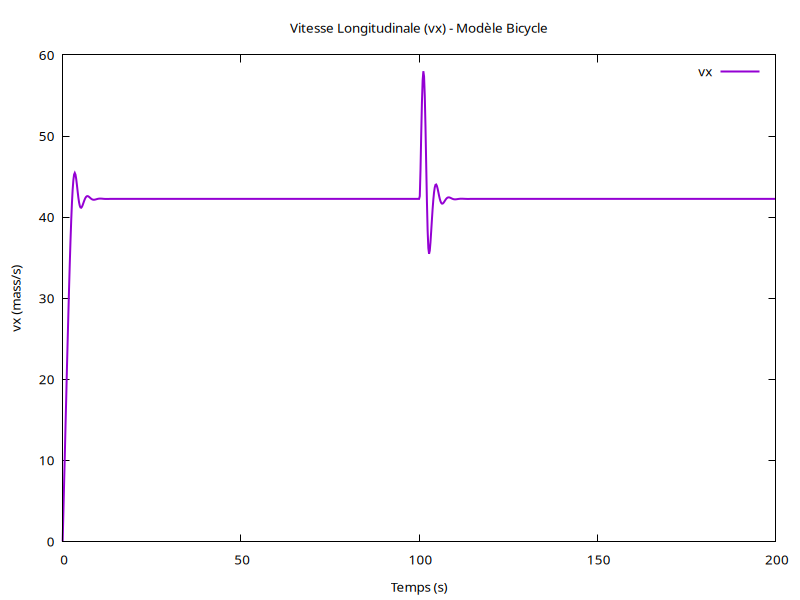
\includegraphics[width=0.70\linewidth]{resources/Plots/Etape2/vx_bicycle}
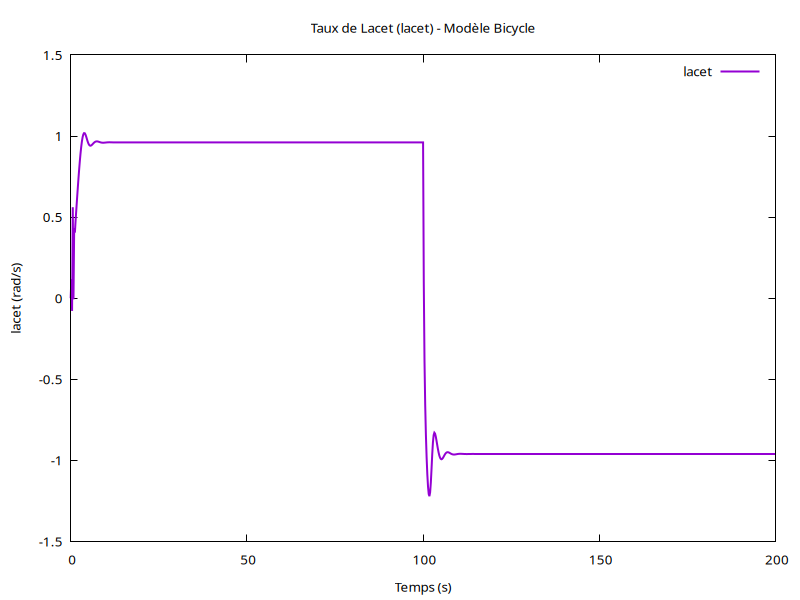
\includegraphics[width=0.70\linewidth]{resources/Plots/Etape2/r_bicycle}
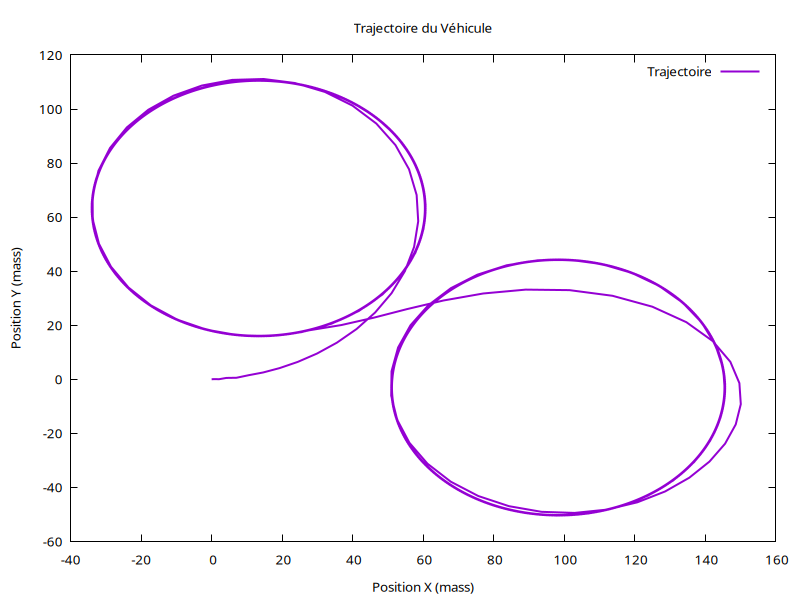
\includegraphics[width=0.70\linewidth]{resources/Plots/Etape2/trajectory}
\end{center}

\subsection{Introduction d'un glissement dynamique}

Comme nous avons vu dans la partie précédente, nous avons introduit un nouveau paramètre, appelé \texttt{slip}, qui représente le glissement entre la surface du pneu et la route. Il influence la force longitudinale générée par le pneu avant. En d'autres termes, il détermine combien de force de traction est appliquée en fonction du glissement effectif entre le pneu et la surface. Cependant, jusqu'à présent, sa valeur était constante ; dans cette partie, nous allons donc nous intéresser à le rendre dynamique.

Une valeur de \texttt{slip} dynamique évolue donc au fil du temps pour atteindre une valeur désirée, car dans la réalité le glissement d'un pneu ne change pas instantanément, mais suit une dynamique bien spécifique. Pour introduire le dynamisme de cette variable, nous devons introduire de nouvelles variables :

\begin{itemize}
\item \texttt{initSlip} : La valeur initiale du slip,

\item \texttt{initSlip\_tau} : La constante de temps qui va déterminer à quelle rapidité \texttt{slip} évolue vers sa valeur cible

\item \texttt{initS\_desired} : La valeur cible du slip que le système cherche à atteindre.

\end{itemize}

Ces nouvelles variables vont donc nous aider à définir le comportement du \texttt{slip} sur une durée.
Une constante de temps \texttt{initSlip\_tau} faible fait que \texttt{slip} atteindra sa valeur cible rapidement, et au contraire une constante de temps élevée induit une réponse plus lente.
Avec toutes ces nouvelles données, nous pouvons donc modéliser la dynamique du \texttt{slip} par une équation du premier ordre :
$$\dot{\texttt{slip}} = \frac{s_{\texttt{desired}} - \texttt{slip}}{\texttt{slip}_{\texttt{desired}}}$$

Cette équation traduit donc le fait que le taux de variation du \texttt{slip} $(\dot{\texttt{slip}})$, est proportionnel à l'écart entre la valeur désirée et la valeur actuelle.
Par la suite, on intègre cette donnée avec la méthode d'Euler pour la mettre à jour, ce qui donne donc dans notre fonction \texttt{updateBicycle} :

\begin{lstlisting}[style=CStyle,label={lst:code_update_bicycle_etape3}]
void updateBicycleEtape3(double dt, double delta) {
    ...
    double slip_dot = (s_desired - slip) / slip_tau;
    slip += slip_dot * dt;
    ...
}
\end{lstlisting}

Ici, on remarque dans la fonction que le paramètre \texttt{slip} n'est plus donné en argument, il est maintenant un argument de notre classe, et est initialisé à une valeur quelconque, puis sa valeur est calculée et change dynamiquement.

\subsection{Limites des pneumatiques}

Grâce aux parties précédentes, nous pouvons donc déterminer la trajectoire d'une voiture, mais nous ne pouvons pas encore représenter et visualiser les phénomènes où la charge maximale des pneumatiques a été dépassée, ce qui mène ensuite à un sous-virage ou survirage. Nous allons donc intégrer les limites physiques des pneumatiques à notre simulation pour représenter la force latérale maximale qu'un pneu peut générer avant de perdre son adhérence. Pour faire cela, nous allons introduire une saturation non linéaire des forces latérales, qui ne peuvent pas fournir une force infinie lors d'un virage.

\subsubsection{Calcul des Charges sur les Essieux}

Pour déterminer la force latérale maximale que peut générer chaque essieu, nous devons déjà connaître la charge verticale des pneus. Ces charges sont obtenues à partir de la répartition du poids du véhicule. Nous utilisons donc les formules suivantes :

\begin{itemize}
\item \textbf{Essieu avant} :
$$F_{z\_front} = m \times g \times \frac{b}{a+b}$$
\item \textbf{Essieu arrière} :
$$F_{z\_rear} = m \times g \times \frac{b}{a+b}$$

Avec :\\
$a$ = Distance entre le \textbf{centre de gravité} et l'\textbf{essieu avant},\\
$b$ = Distance entre le \textbf{centre de gravité} et l'\textbf{essieu arrière},\\
$m$ = La masse du véhicule, \\
$g$ = La constante gravitationnelle \\
%%\center{\text{(Formules tirées de \cite{axle_weights})}} % TODO create bib entry
\end{itemize}

Avec ces forces verticales, nous pouvons ensuite déterminer les forces latérales maximales en fonction des coefficients de friction. Ces forces sont notées $F_{y, max}$ et sont calculées en multipliant la charge verticale par le coefficient d'adhérence propre à chaque essieu. Le coefficient d'adhérence des pneus avant et arrières est représenté respectivement par $\mu_{\texttt{front}}$ et $\mu_{\texttt{rear}}$. Grâce à ceux-ci, nous pouvons donc également modifier la capacité des pneus à générer de l'adhérence. Une valeur fixée à $0.9$, représentera ainsi une route mouillée, à $0.7$ une route mouillée. Plus on monte sa valeur, plus le véhicule arrive à générer une force d'adhérence avec le revêtement, et contrairement, plus sa valeur est faible, moins d'adhérence est générée.

\begin{itemize}
    \item \textbf{Essieu avant} :
    $$F_{y\_\texttt{max\_front}}= \mu_{\texttt{front}} \times F_{z\_\texttt{front}}$$
    \item \textbf{Essieu arrière} :
    $$F_{y\_\texttt{max\_rear}} = \mu_{\texttt{rear}} \times F_{z\_\texttt{rear}}$$
\end{itemize}

Premièrement, nous calculons les forces latérales, on rappelle que la formule est la suivante :

\begin{itemize}
    \item \texttt{F\_y\_front} : $$2 \times C_y \times \alpha_F$$
    \item \texttt{F\_y\_rear} : $$2 \times C_y \times \alpha_R$$
\end{itemize}

Cependant, à ce moment-ci, elles sont linéaires et, pour les différencier des forces finales, on les notera : \texttt{F\_y\_front\_linear} et \texttt{F\_y\_rear\_linear}. Maintenant, pour tenir compte de l'adhérence limitée, nous définissons deux rapports :

\begin{align}
    \texttt{ratio\_front} &= \frac{\texttt{F\_y\_front}}{\texttt{F\_y\_front\_max}} \\
    \texttt{ratio\_rear} &= \frac{\texttt{F\_y\_rear}}{\texttt{F\_y\_rear\_max}}
\end{align}

Ensuite, nous pouvons utiliser ce rapport pour modéliser la saturation. Ainsi, la force latérale effective est donnée par :

\begin{itemize}
    \item \texttt{F\_y\_front} : $$\texttt{F\_y\_max\_front} \times \tanh(\texttt{ratio\_front})$$
    \item \texttt{F\_y\_rear} : $$\texttt{F\_y\_max\_rear} \times \tanh(\texttt{ratio\_rear})$$
\end{itemize}

Ici, nous utilisons la fonction $\tanh$, car elle se comporte de manière linéaire pour des faibles valeurs de ratios, et elle tend vers une valeur asymptomatique $(1)$ lorsque le ratio augmente, ce qui limite la force latérale. À terme, la force d'adhérence générée par le pneu ne peut pas dépasser sa limite. Grâce à ces nouvelles limites, nous pouvons donc simuler la saturation des pneumatiques, ce qui nous permet d'éviter d'avoir des forces latérales irréalistes dans notre simulation. Mais également de reproduire le phénomène de survirage et de sous-virage, en effet quand la force latérale requise dépasse la limite d'adhérence, le véhicule ne peut pas suivre la trajectoire désirée.

Cependant, nous avons rencontré un problème fondamental en essayant de faire fonctionner notre simulation, la précision et la stabilité numérique des équations différentielles de notre système nous donnaient des valeurs totalement incohérentes. Après une grande analyse des différents systèmes implémentés dans notre modèle, nous avons compris que c'était notre utilisation de la méthode d'Euler. Après avoir fait des tests approfondis, nous avons constaté que cette approche générait des erreurs significatives qui compromettaient totalement la fidélité de notre modèle. Après avoir réétudié la méthode d'Euler, nous avons compris qu'elle n'était plus adaptée, car elle introduit une erreur d'approximation, en particulier lorsque le système présente des dynamiques rapides ou non linéaires. Dans notre cas, plusieurs phénomènes incohérents sont apparus lors des simulations :
\begin{itemize}
    \item Des oscillations dans les trajectoires,
    \item Une instabilité totale de toutes les données pour des pas de temps trop élevés,
    \item Une divergence des valeurs dans certaines conditions.
\end{itemize}
Ce tout rendait notre modèle totalement inutilisable, nous avons donc décidé d'explorer différentes alternatives d'intégration numérique. Après une recherche étoffée, nous avons décidé d'utiliser une méthode d'intégration plus avancée : \textbf{Runge-Kutta d'ordre 4 (RK4}. En effet, RK4 s'est révélée être un compromis idéal entre précision et performance. Contrairement à la méthode d'Euler qui se base sur une seule estimation du taux de variation, RK4 effectue plusieurs évaluations intermédiaires pour améliorer la précision. Elle suit le schéma suivant :

\begin{align}
    k_1 &= f(x_n+t_n)\\
    k_2 &= f(x_n+ {\frac{h}{2}}k_1, t_n + {\frac{h}{2}})\\
    k_3 &= f(x_n+ {\frac{h}{2}}k_2, t_n + {\frac{h}{2}})\\
    k_4 &= f(x_n+ hk_3, t_n + h)
\end{align}
\begin{center}
    Formule disponible sur : \cite{RK4}
\end{center}
Concrètement RK4 repose sur quatre évaluations intermédiaires $(k_1, \ k_2, \ k_3, \ k_4)$ qui correspondent aux
dérivées estimées du système à différents instants au sein d'un même pas de temps. Dans notre cas, ces dérivées
représentent les variations des états dynamiques du véhicule qui comprennent :

\begin{itemize}
    \item La position $(x,y)$,
    \item L'orientation $(\theta)$,
    \item Les vitesses longitudinales et latérales $(v_x, v_y)$,
    \item La vitesse angulaire $(\omega)$.
\end{itemize}

Ce processus nous permet d'obtenir une estimation correcte, réduisant l'erreur d'approximation de $O(h^2)$ à $O(h^4)$,
ce qui restaure la stabilité et la fidélité du modèle. Avec cette étape du modèle, qui est la dernière, nous pouvons
donc observer différentes trajectoires, et en particulier, nous pouvons bien observer le phénomène de sous-virage.

Après avoir produit une physique qui suffisait à notre simulateur, nous avons décidé d'utiliser Gnuplot pour pouvoir
afficher  les données produites par notre modèle, et ainsi pouvoir visualiser les réactions des différents paramètres
utilisés dans notre simulation.
Tout ceci est géré dans notre fichier \texttt{plotting.cpp}, et gr�ce a notre classe \texttt{vehicule.cpp}, et sa
fonction

